\documentclass{article}
\usepackage{indentfirst}
\usepackage{listings}
\usepackage{amsmath}
\usepackage{amssymb}
\usepackage{amsthm}
\usepackage{url}
\usepackage{tikz-cd}
\usepackage[utf8]{inputenc}

\setlength{\parindent}{15pt}

\theoremstyle{definition}
\newtheorem{theorem}{Theorem}
\newtheorem{definition}{Definition}

\lstset{basicstyle=\footnotesize,inputencoding=utf8,
literate=
{𝟎}{{\ensuremath{\mathbf{0}}}}1
{𝟏}{{\ensuremath{\mathbf{1}}}}1
{≔}{{\ensuremath{\mathrm{:=}}}}1
{α}{{\ensuremath{\mathrm{\alpha}}}}1
{ᵂ}{{\ensuremath{^W}}}1
{β}{{\ensuremath{\mathrm{\beta}}}}1
{γ}{{\ensuremath{\mathrm{\gamma}}}}1
{δ}{{\ensuremath{\mathrm{\delta}}}}1
{ε}{{\ensuremath{\mathrm{\varepsilon}}}}1
{ζ}{{\ensuremath{\mathrm{\zeta}}}}1
{η}{{\ensuremath{\mathrm{\eta}}}}1
{θ}{{\ensuremath{\mathrm{\theta}}}}1
{ι}{{\ensuremath{\mathrm{\iota}}}}1
{κ}{{\ensuremath{\mathrm{\kappa}}}}1
{λ}{{\ensuremath{\mathrm{\lambda}}}}1
{μ}{{\ensuremath{\mathrm{\mu}}}}1
{ν}{{\ensuremath{\mathrm{\nu}}}}1
{ξ}{{\ensuremath{\mathrm{\xi}}}}1
{π}{{\ensuremath{\mathrm{\mathnormal{\pi}}}}}1
{ρ}{{\ensuremath{\mathrm{\rho}}}}1
{σ}{{\ensuremath{\mathrm{\sigma}}}}1
{τ}{{\ensuremath{\mathrm{\tau}}}}1
{φ}{{\ensuremath{\mathrm{\varphi}}}}1
{χ}{{\ensuremath{\mathrm{\chi}}}}1
{ψ}{{\ensuremath{\mathrm{\psi}}}}1
{ω}{{\ensuremath{\mathrm{\omega}}}}1
{Π}{{\ensuremath{\mathrm{\Pi}}}}1
{Γ}{{\ensuremath{\mathrm{\Gamma}}}}1
{Δ}{{\ensuremath{\mathrm{\Delta}}}}1
{Θ}{{\ensuremath{\mathrm{\Theta}}}}1
{Λ}{{\ensuremath{\mathrm{\Lambda}}}}1
{Σ}{{\ensuremath{\mathrm{\Sigma}}}}1
{Φ}{{\ensuremath{\mathrm{\Phi}}}}1
{Ξ}{{\ensuremath{\mathrm{\Xi}}}}1
{Ψ}{{\ensuremath{\mathrm{\Psi}}}}1
{Ω}{{\ensuremath{\mathrm{\Omega}}}}1
{ℵ}{{\ensuremath{\aleph}}}1
{≤}{{\ensuremath{\leq}}}1
{≥}{{\ensuremath{\geq}}}1
{≠}{{\ensuremath{\neq}}}1
{≈}{{\ensuremath{\approx}}}1
{≡}{{\ensuremath{\equiv}}}1
{≃}{{\ensuremath{\simeq}}}1
{≤}{{\ensuremath{\leq}}}1
{≥}{{\ensuremath{\geq}}}1
{∂}{{\ensuremath{\partial}}}1
{∆}{{\ensuremath{\triangle}}}1 % or \laplace?
{∫}{{\ensuremath{\int}}}1
{∑}{{\ensuremath{\mathrm{\Sigma}}}}1
{→}{{\ensuremath{\rightarrow}}}1
{⊥}{{\ensuremath{\perp}}}1
{∞}{{\ensuremath{\infty}}}1
{∂}{{\ensuremath{\partial}}}1
{∓}{{\ensuremath{\mp}}}1
{±}{{\ensuremath{\pm}}}1
{×}{{\ensuremath{\times}}}1
{⊕}{{\ensuremath{\oplus}}}1
{⊗}{{\ensuremath{\otimes}}}1
{⊞}{{\ensuremath{\boxplus}}}1
{∇}{{\ensuremath{\nabla}}}1
{√}{{\ensuremath{\sqrt}}}1
{⬝}{{\ensuremath{\cdot}}}1
{•}{{\ensuremath{\cdot}}}1
{∘}{{\ensuremath{\circ}}}1
{⁻}{{\ensuremath{^{-}}}}1
{▸}{{\ensuremath{\blacktriangleright}}}1
{∧}{{\ensuremath{\wedge}}}1
{∨}{{\ensuremath{\vee}}}1
{¬}{{\ensuremath{\neg}}}1
{⊢}{{\ensuremath{\vdash}}}1
{⟨}{{\ensuremath{\langle}}}1
{⟩}{{\ensuremath{\rangle}}}1
{↦}{{\ensuremath{\mapsto}}}1
{→}{{\ensuremath{\rightarrow}}}1
{↔}{{\ensuremath{\leftrightarrow}}}1
{⇒}{{\ensuremath{\Rightarrow}}}1
{⟹}{{\ensuremath{\Longrightarrow}}}1
{⇐}{{\ensuremath{\Leftarrow}}}1
{⟸}{{\ensuremath{\Longleftarrow}}}1
{∩}{{\ensuremath{\cap}}}1
{∪}{{\ensuremath{\cup}}}1
{⊂}{{\ensuremath{\subseteq}}}1
{⊆}{{\ensuremath{\subseteq}}}1
{⊄}{{\ensuremath{\nsubseteq}}}1
{⊈}{{\ensuremath{\nsubseteq}}}1
{⊃}{{\ensuremath{\supseteq}}}1
{⊇}{{\ensuremath{\supseteq}}}1
{⊅}{{\ensuremath{\nsupseteq}}}1
{⊉}{{\ensuremath{\nsupseteq}}}1
{∈}{{\ensuremath{\in}}}1
{∉}{{\ensuremath{\notin}}}1
{∋}{{\ensuremath{\ni}}}1
{∌}{{\ensuremath{\notni}}}1
{∅}{{\ensuremath{\emptyset}}}1
{∖}{{\ensuremath{\setminus}}}1
{†}{{\ensuremath{\dag}}}1
{ℕ}{{\ensuremath{\mathbb{N}}}}1
{ℤ}{{\ensuremath{\mathbb{Z}}}}1
{ℝ}{{\ensuremath{\mathbb{R}}}}1
{ℚ}{{\ensuremath{\mathbb{Q}}}}1
{ℂ}{{\ensuremath{\mathbb{C}}}}1
{⌞}{{\ensuremath{\llcorner}}}1
{⌟}{{\ensuremath{\lrcorner}}}1
{⦃}{{\ensuremath{ \{\!| }}}1
{⦄}{{\ensuremath{ |\!\} }}}1
{₁}{{\ensuremath{_1}}}1
{₂}{{\ensuremath{_2}}}1
{₃}{{\ensuremath{_3}}}1
{₄}{{\ensuremath{_4}}}1
{₅}{{\ensuremath{_5}}}1
{₆}{{\ensuremath{_6}}}1
{₇}{{\ensuremath{_7}}}1
{₈}{{\ensuremath{_8}}}1
{₉}{{\ensuremath{_9}}}1
{₀}{{\ensuremath{_0}}}1
{¹}{{\ensuremath{^1}}}1
{ₙ}{{\ensuremath{_n}}}1
{ₘ}{{\ensuremath{_m}}}1
{↑}{{\ensuremath{\uparrow}}}1
{↓}{{\ensuremath{\downarrow}}}1
{▸}{{\ensuremath{\triangleright}}}1
{∀}{{\ensuremath{\forall}}}1
{∃}{{\ensuremath{\exists}}}1
{λ}{{\ensuremath{\mathrm{\lambda}}}}1
{=}{{\ensuremath{=}}}1
{<}{{\ensuremath{\langle}}}1
{>}{{\ensuremath{\rangle}}}1
{(}{(}1
{(}{(}1
{‖}{‖}1
{+}{{+}}1
{*}{{*}}1,
}

\begin{document}

\title{Issue VI: The Arthur Language}
\author{Maksym Sokhatskyi $^1$}
\date{ $^1$ National Technical University of Ukraine \\
       \small Igor Sikorsky Kyiv Polytechnical Institute \\
       \today }

\maketitle

\begin{abstract}

Minimal language for parallel computations in symmetric monoidal categories. \\
{\bf Keywords}: Interaction Networks, Symmetric Monoidal Categories
\end{abstract}

\ifincludeTOC
  \tableofcontents
\fi

\newpage

\epigraph{Присвячується автору K}{Артуру Вітні}

Третій розділ описує розвиток концептуальної моделі системи доведення теорем як сукупності
формальних середовищ виконання, кожне наступе з яких, складніше за попереднє,
має свою операційну семантику, та наслідує усі властивості попередніх операційних середовищ послідовності.

\section{The Arthur Language}

Мінімальна мова системи $O_{CPS_\lambda}$ визначається простим
синтаксичним деревом:

\begin{lstlisting}
def CPS$_\lambda$ : U
 := inductive { var (x: nat)
              | lam (l: nat) (d: cps)
              | app (f a: cps)
              }
\end{lstlisting}

Однак, на практиці, застосовують більш складні описи синтаксичних дерев,
зокрема для лінивих обчислень, та розширення синтаксичного дерева спеціальними
командами пов'язаними з середовищем виконання. Програми таких
інтерпретаторів відповідно виконуються у певній пам'яті, яка
використовується як контекст виконання. Кожна така програма крутиться
як одиниця виконання на певному ядрі процесора. Ситема процесів, де
кожен процес є CPS-програмою яку виконує інтерпретатор на певному ядрі.

Мотивація для побудови такого інтерпретатору, який повністю розміщується
разом зі программою в L1 стеку (який лімітований 64КБ) базується на успіху
таких віртуальних машин як LuaJIT, V8, HotSpot, а також векторних мов
програмування типу К та J. Якби ми могли побудувати дійсно швидкий інтерпретатор
який би виконував програми цілком в L1 кеші, байткод та стріми якого були би
вирівняні по словам архітектури, а для векторних обчислень застосовувалися би AVX інструкції,
які, як відомо перемагають по ціні-якості GPU обчислення. Таким чином, такий
інтерпретатор міг би, навіть без спеціалізованої JIT компіляції, скласти
конкуренцію сучасним промисловим інтерпретаторам, таким як Erlang, Python, K, LuaJIT.

\begin{table}
 \caption{Заміри на інтерпретаторах ландшафту атаки}
  \begin{tabular}{rc}
    \hline
\rowcolor{ZimaBlue}
    \textbf{Мова} & \textbf{Fac(5) в нс} \\
    \hline
    Rust    & 0 \\
    Java    & 3 \\
    PyPy    & 8 \\
    \hline
    \rowcolor{LightGray}
    CPS     & 291 \\
    \hline
    Python  & 537 \\
    K       & 756/635 \\
    \hline
    \rowcolor{LightGray}
    Erlang  & 10699/1806/436/9 \\
    \hline
    LuaJIT  & 33856 \\
    \hline
  \end{tabular}
\end{table}

Для дослідження цієї гіпотези мною було побудовано еспериментальний інтерпретатор
без байт-коду, але з вирівняним по словам архітерктури стріму команд, які є
безпосередньою машинною презентацією конструкторів індуктивних типів (enum) мови Rust.
Наступні результати були отримані після неотпимізованої версії інтерпретатора
при обчисленні факторіала (5) та функції Акермана у точці (3,4).

\begin{table}
 \caption{Заміри на інтерпретаторах ландшафту атаки}
  \begin{tabular}{rc}
    \hline
\rowcolor{ZimaBlue}
    \textbf{Мова} & \textbf{Akk(3,4) в мкс} \\
    \hline
    \rowcolor{LightGray}
CPS & 635 \\
    \hline
Rust  & 8,968 \\
    \hline
  \end{tabular}
\end{table}

Ключовим викликом тут стали лінійні типи мови Rust, які не дозволяють
звертатися до ссилок, які вже були оброблені, а це впливає на всю
архітектуру тензорного преставлення змінних в мові інтерпретатор $O_{CPS}$,
яка наслідує певним чином мову К.

\newpage
\subsection{Векторизація засобами мови Rust}

\begin{lstlisting}
objdump ./target/release/o -d | grep mulpd
   223f1: c5 f5 59 0c d3    vmulpd (%rbx,%rdx,8),%ymm1,%ymm1
   223f6: c5 dd 59 64 d3 20 vmulpd 0x20(%rbx,%rdx,8),%ymm4,%ymm4
   22416: c5 f5 59 4c d3 40 vmulpd 0x40(%rbx,%rdx,8),%ymm1,%ymm1
   2241c: c5 dd 59 64 d3 60 vmulpd 0x60(%rbx,%rdx,8),%ymm4,%ymm4
   2264d: c5 f5 59 0c d3    vmulpd (%rbx,%rdx,8),%ymm1,%ymm1
   22652: c5 e5 59 5c d3 20 vmulpd 0x20(%rbx,%rdx,8),%ymm3,%ymm3
\end{lstlisting}

\subsection{Байт-код інтерпретатора}
Синтаксичне дерево, або неформалізований бай-код віртуальної
машини або інтерпретатора $O_{CPS}$ розкладається на два дерева, одне дерево
для управляючих команд інтерпретатора: Defer, Continuation, Start (початок програми),
Return (завершення програми).

\begin{lstlisting}
def Lazy : U
 := inductive { Defer (otree: NodeId) (a: AST) (cont: Cont)
              | Continuation (otree: NodeId) (a: AST) (cont: Cont)
              | Return (a: AST)
              | Start
              }
\end{lstlisting}

Операції віртуальної машини: умовний оператор, оператор присвоєння, лямбда
функція та аплікація, є відображеннями на конструктори синтаксичного дерева.

\begin{lstlisting}
def Cont : U
 := inductive { Expressions (a: AST) (v: Option (Iter AST)) (c: Cont)
              | Assign (ast: AST) (cont: Cont)
              | Cond (c,d: AST) (cont: Cont)
              | Func (a,b,c: AST) (cont: Cont)
              | List (acc: Vec AST) (vec: Iter AST) (i: Nat) (c: Cont)
              | Call (a: AST) (i: Nat) (cont: Cont)
              | Return
              | Intercore (m: Message) (cont: Cont)
              | Yield (cont: Cont)
              }
\end{lstlisting}

\newpage
\subsection{Синтаксис}
Синтаксис мови $O_{CPS}$ підтримує тензори, та звичайне лямбда числення
з значеннями у тензорах машинних типів даних: i32, i64.

\begin{lstlisting}[mathescape=true]
E: V | A | C
NC: ";" = [] | ";" m:NL = m
FC: ";" = [] | ";" m:FL = m
EC: ";" = [] | ";" m:EL = m
NL: NAME | o:NAME m:NC = Cons o m
FL: E | o:E | m:FC = Cons o m
EL: E | EC  | o:E m:EC = Cons o m
C: N | c:N a:C = Call c a
N: NAME | S | HEX | L | F
L: "(" ")" = [] | "([" c:NL "]" m:FL ")" = Table c m
                | "(" l:EL ")" = List l
F: "{" "}" = Lambda [] [] []
           | "{[" c:NL "]" m:EL "}" = Lambda [] c m
           | "{" m:EL "}" = Lambda [] [] m
\end{lstlisting}

Після парсера, синтаксичне дерево розкладається по наступним складовим: AST для
тензорів (визначення вищого рівня); Value для машинних слів; Scalar для
конструкцій мови (куди входить зокрема списки та словники, умовний оператор,
присвоєння, визначення функції та її аплікація, UTF-8 літерал, та оператор
передачі управління в поток планувальника який закріплений за певним ядром CPU).

\begin{lstlisting}
def AST : U
 := inductive { Atom (a: Scalar)
              | Vector (a: Vec AST)
              }
\end{lstlisting}

\begin{lstlisting}
def Value : U
 := inductive { Nil
              | SymbolInt (a: u16)
              | SequenceInt (a: u16)
              | Number (a: i64)
              | Float (a: f64)
              | VecNumber (Vec i64)
              | VecFloat (Vec f64)
              }
\end{lstlisting}

\newpage
\begin{lstlisting}
def Scalar : U
 := inductive { Nil
              | Any
              | List (a: AST)
              | Dict (a: AST)
              | Call (a b: AST)
              | Assign (a b: AST)
              | Cond (a b c: AST)
              | Lambda (otree: Option NodeId) (a b: AST)
              | Yield (c: Context)
              | Value (v: Value)
              | Name (s: String)
              }
\end{lstlisting}

Кожна секція цієї глави буде присвячена цим мовним компонентам
системи доведення теорем. В кінці розділу дається повна система, яка включає в себе усі
мови та усі мовні перетворення.

\subsection{Система числення процесів SMP async}

\subsubsection{Операційна система}
Перелічимо основні властивості операційної системи (прототип
якої опублікований на Github\footnote{\url{https://github.com/voxoz/kernel}}).

\textbf{Властивості}: автобалансована низьколатентна, неблокована, без копіювання, система черг
з CAS-мультикурсорами, з пріоритетами задач та масштабованими таймерами.

\subsubsection{Асиметрична багапроцесорність}
Ядро системи використовує асиметричну багапроцесорність (АП)
для планування машинного часу. Так у системі для консольного
вводу-виводу та вебсокет моніторингу використовується окремий
ректор (закріплений за ядром процессора),
аби планування не впливало на програми на інших процесорах.

\newpage
Це означає статичне закріплення певного атомарного процесу
обчислення за певним реактором, та навіть можливо дати гарантію, що
цей процес не перерветься при наступному кванті планування
ніяким іншим процесом на цьому ядрі (ситуація єдиного процесу
на реактор ядра процесору). Ядро системи постачається разом з конфігураційною
мовою для закріплення задач за реакторами:

\begin{lstlisting}
reactor[aux;0;mod[console;network]];
reactor[timercore;1;mod[timer]];
reactor[core1;2;mod[task]];
reactor[core2;3;mod[task]];
\end{lstlisting}

\subsubsection{Низьколатентність}
Усі реактори повинні намагатися обмежити IP-лічильник команд
діапазоном розміром з L1/L2 кеш об'єм процесора, для унеможливлення
колізій між ядрами на міжядерній шині можлива конфігурація, де
реактори виконують код, області пам'яті якого не перетинаються,
та обмежені об'ємом L1 кеш пам'яті що при наявній AVX векторизації
дать змогу повністю використовувати ресурси процесору наповну.

\newpage
\subsubsection{Мультикурсори}
Серцем низьколатентної системи транспорту є система наперед виділений
кільцевих буферів (які називаються секторами глобального кільця). У цій
системі кілець діє система курсорі для запису та читання, ці курсори
можуть мати різний напрямок руху.
\begin{figure}[ht]
  \centerline{\includegraphics[scale=0.25]{pub.eps}}
  \caption{Кільцева статична черга з CAS-курсором для публікації}
\end{figure}
Для забезпечення імутабельності (нерухомості даних) та відсутності
копіювання в подальшій роботі, дані залишаються в черзі, а рухаються та передаються
лише курсори на типизовані послідовності даних.
\begin{figure}[ht]
  \centerline{\includegraphics[scale=0.25]{sub.eps}}
  \caption{Кільцева статична черга з CAS-курсором для згортки}
\end{figure}

\newpage
\subsubsection{Реактори}
Кожен процесор має три типи реакторів які можуть бути на ньому запущені:
i) Task-реактор; ii) Timer-реактор; iii) IO-цикли. Для Task-реактора
існують черги пріорітетів, а для Timer-реактора --- дерева інтервалів.
\begin{figure}[ht]
  \captionsetup{justification=raggedright,singlelinecheck=false}
  \centerline{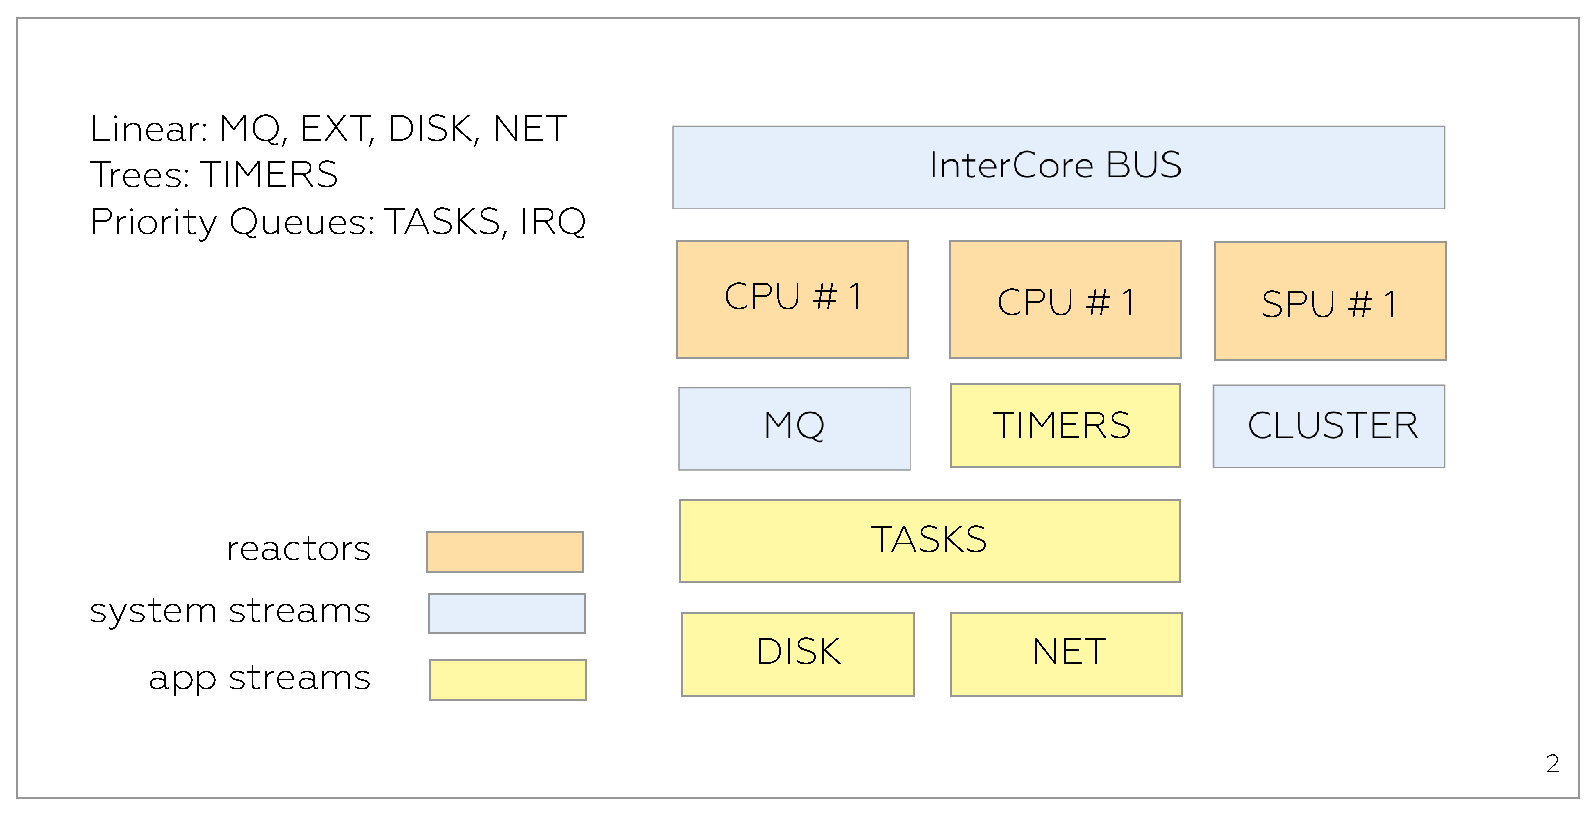
\includegraphics[scale=0.25]{sys.eps}}
  \caption{Система процесорних ядер та реакторів}
\end{figure}
Загальний спосіб комунікації для задач виглядає як публікація
у чергу (рух курсора запису) та підписка на черги і
згортання (руху курсора читання). Кожна черга має як
курсори для публікації так і курсори для читання. Можливо також
використання міжреакторної шини InterCore та посилання
службового повідомлення по цій шині на інший реактор. Так,
наприклад, працюють таймери та старти процесів, які передають
сигнал в реактор для перепланування. Можна створювати нові повідомлення
шини InterCore і систему фільтрів для згортання черги
реактора для більш гнучкої обробки сигналів реального часу.

\subsubsection*{Task-реактор}
Task-реактор або реактор задач виконує Rust задачі або
програми інтерпретатора, які можуть бути двох видів:
кінечні (які повертають результат виконання),
або нескінченні (процеси).
%\begin{figure}[ht]
%  \centerline{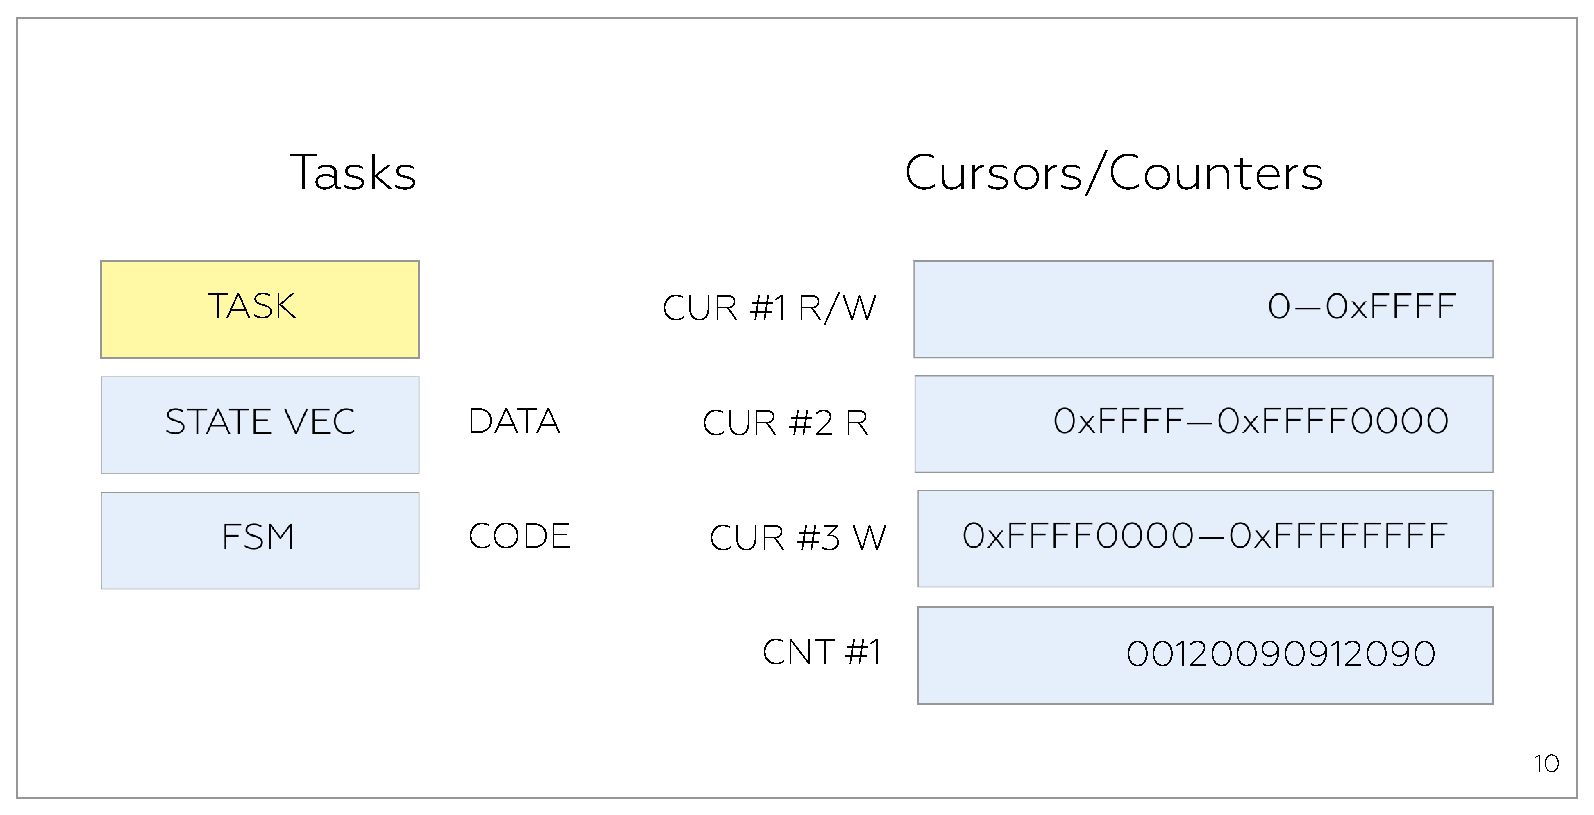
\includegraphics[scale=0.25]{task.eps}}
%  \caption{Task-реактор або система інтерпретаторів}
%\end{figure}

Приклад бескінечної задачі --- 0-процес,
який запускається при старті системи. Цей процес завжди доступний
по WebSocket каналу та з консолі терміналу.

\subsubsection*{IO-реактор}
Мережевий сервер або IO-реактор може обслуговувати багато
мережевих з'єднань та підтримує Windows, Linux, Mac смаки.
%\begin{figure}[ht]
%  \centerline{\includegraphics[scale=0.25]{net.eps}}
%  \caption{IO-реактор або процес опитування мережевих сервісів}
%\end{figure}

\subsubsection*{Timer-реактор}
Різні типи сутностей планування (такі як Task, IO, Timer)
мають різні дисципліни селекторів повідомлень для черг
(послідовно, через само-балансуючі дерева, BTree дерева тощо).
%\begin{figure}[ht]
%  \centerline{\includegraphics[scale=0.25]{timer.eps}}
%  \caption{Timer-реактор або драйвер процесорного таймеру}
%\end{figure}

\subsubsection{Міжреакторний транспорт InterCore}
Шина InterCore конструюється певним числом SPMC черг, виділених для певного ядра.
Шина сама має топологію зірки між ядрами, та черга MPSC організована
як функція над множиною паблішерів. Кожне ядро має рівно одного паблішера.
Функція обробки шини протоколу InterCore називається poll\_bus та є членом планувальника.
Ви можете думати про InterCore як телепорт між процесорами, так як pull\_bus
викликається після кожної операції Yield в планувальник, і, таким чином,
якщо певному ядру опублікували в його чергу повідомлення, то після наступного Yield
на цьому ядрі буде виконана функція обробки цього повідомлення.

\subsubsection*{\lstinline{fun pub(capacity: int): int}}
Створює новий CAS курсор для паблішінга, тобто для запису.
Повертає глобальних машинний ідентифікатор, має єдиний параметр, розмір черги.
Приклад: p: pub[16].

\subsubsection*{\lstinline{fun sub(publisher: int): int}}
Створює новий CAS курсор для читання певної черги, певного врайтера.
Повертає глобальний машинний ідентифікатор для читання.
Приклад: s: sub[p].

\subsubsection*{\lstinline{fun spawn(core: int, program: code, cursors: array int): int}}
Створює нову програму задачу CPS-інтепреторатора для певного ядра.
Задача може бути або програмою на мові Rust або будь якою програмою через FFI.
Також при створенні задачі задається список курсорів,
які ексклюзивно належатимуть до цієї задачі.
Параметри функції: ядро, текст програми або назва FFI функції,спсисок курсорів.

\subsubsection*{\lstinline{fun kill(process: int): int}}
Денонсація процесора на реаторі.

\subsubsection*{\lstinline{fun send(writer: int, data: binary): int}}
Посилає певні дані в певний курсор для запису. Повертає Nil якшо всьо ОК.
Приклад: snd[p;42].

\subsubsection*{\lstinline{fun receive(reader: int)}}
Повертає прочитані дані з певного курсору.
Якшо даних немає, то передає управління в планувальних за допомогою Yield.
Приклад: rcv[s].

\newpage
\subsection{Структури ядра}
Ядро є ситемою акторів з двома основними типами акторів:
чергами, які представляють кільцеві буфери та відрізки памяті;
та задачами, які резпрезентують байт-код програм та іх інтерпретацію на процесорі.
Черги бувають двох видів: для публікації, які місять курсори для запису;
та для читання, які містять курсори для читання. Задачі можна імплементувати
як Rust програми, або як $O_{CPS}$ програми.

\subsubsection{Черга для публікації}
\begin{lstlisting}
pub struct Publisher<T> {
    ring: Arc<RingBuffer<T>>,
    next: Cell<Sequence>,
    cursors: UncheckedUnsafeArc<Vec<Cursor>>,
}
\end{lstlisting}

\subsubsection{Черга для читання}
\begin{lstlisting}
pub struct Subscriber<T> {
    ring: Arc<RingBuffer<T>>,
    token: usize,
    next: Cell<Sequence>,
    cursors: UncheckedUnsafeArc<Vec<Cursor>>,
}
\end{lstlisting}

Існує дві спецільні задачі: InterCore задача, написана на Rust,
яка запускається на всіх ядрах при запуску системи, а також CPS-інтерпретор
головного термінала системи, який запускається на BSP ядрі, поближче до Console та WebSocket IO селекторів.
В процесі життя різні CPS та Rust задачі можуть бути запущені в такій системі,
поєднуючи гнучкість програм інтерпретатора, та низькорівневих програм, написаних на мові Rust.

Окрім черг та задач, в системі присутні також таймери та інші IO задачі,
такі як сервери мережі або сервери доступу до файлів. Також існують
структури які репрезентують ядра та містять палнувальники.
Уся віртуальна машина є сукупністю таких структур-ядер.

\newpage
\subsubsection{Канал}
Канал складається з одного курсору для запису та багатьох курсорів для читання.
Канал предствляє собою компонент зірки шини InterCore.
\begin{lstlisting}
pub struct Channel {
    publisher: Publisher<Message>,
    subscribers: Vec<Subscriber<Message>>,
}
\end{lstlisting}


\subsubsection{Черги ядра}
Память репрезентує усі наявні черги для публікації та читання на ядрі.
Ця інформація передається клонованою кожній задачі планувальника на цьому ядрі.
\begin{lstlisting}
pub struct Memory<'a> {
    publishers: Vec<Publisher<Value<'a>>,
    subscribers: Vec<Subscriber<Value<'a>>>,
}
\end{lstlisting}

\subsubsection{Планувальник}
Планувальник репрезентує ядра процесара,
які розрізняються як BSP-ядра (або 0-ядра, bootstrap)
та AP ядра (інші ядра > 0, application). BSP ядро
тримає на собі Console та WebSocket IO селектори.
Це означає, що BSP ядро дає свій час на обробку зовнішньої інформації,
у той час як AP процесори не обтяжені
таким навантаженням (io черга в таких планувальниках пуста).
Існує InterCore повідомлення яке додає або видаляє довільні IO селектори
в планувальних для довільних конфігурацій.

\begin{lstlisting}
pub struct Scheduler<'a> {
    pub tasks: Vec<T3<Job<'a>>>,
    pub bus: Channel,
    pub queues: Memory<'a>,
    pub io: IO,
}
\end{lstlisting}

\newpage
\subsubsection{Протокол InterCore}
Протокол шини InterCore.

\begin{lstlisting}
pub enum Message {
    Pub(Pub),
    Sub(Sub),
    Print(String),
    Spawn(Spawn),
    AckSub(AckSub),
    AckPub(AckPub),
    AckSpawn(AckSpawn),
    Exec(usize, String),
    Select(String, u16),
    QoS(u8, u8, u8),
    Halt,
    Nop,
}
\end{lstlisting}

\subsection{Система числення тензорів AVX}
Для реалізації мови програмування високого рівня на BLAS Level 3 бекендом
була вибрана мова NumLin, серед інших: 1) Ling, 2) Guarded Cubical,
3) A Fibrational Framework for Substructural and Modal Logics,
4) APL-like interpreter in Rust (дана робота), 5) Futhark.

\begin{lstlisting}
def AVX-512 : U
 := inductive { Star | True | False
              | Variable (_: Var)
              | Prim (_: Builtin)
              | Int (_: nat) | Float (_: float)
              | Lambda (a: Var) (b: Linear) (c: Exp)
              | App (a b: Exp)
              | Pair (a b: Var) (c d: Exp)
              | Consume (a: Var) (b c: Exp)
              | Gen (a: Var) (b: Exp)
              | Spec (a: Exp) (b: Fraction)
              | Fix (a b: Var) (c d: Linear) (e: Exp)
              | If (a b c: Exp)
              | Let (a: Var) (b c: Exp)
              }
\end{lstlisting}

\subsection{Висновки}
Перша стадія реалізації класичного лінивого інтерпретатора з CPS семантикою
була виконана як MVP трейдингової HFT платформи. Наступна стадія — виконання
верифікованого інтерпретатора (віртуальної машини) та компілятора (в неї) Standard ML мови на
основі компілятора Joe (MinCaml).

\end{document}